\documentclass[border=10pt]{standalone}
\usepackage{tikz}\usepackage{amsmath}\usetikzlibrary{arrows.meta}
\begin{document}
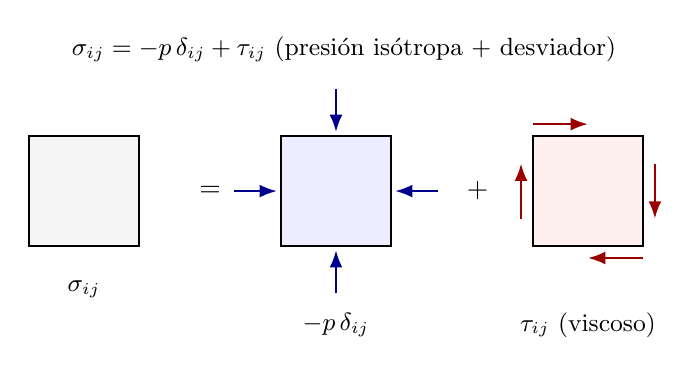
\begin{tikzpicture}[line width=0.9pt,>={Latex[length=2.2mm]}]
  \draw[fill=black!4] (0,0) rectangle (1.4,1.4);
  \node at (0.7,-0.55){\small $\sigma_{ij}$};
  \node at (2.3,0.7){$=$};
  % presion isotropa: flechas hacia adentro en las 4 caras
  \draw[fill=blue!7] (3.2,0) rectangle (4.6,1.4);
  \draw[->,blue!55!black] (3.9,2.0)--(3.9,1.45);
  \draw[->,blue!55!black] (3.9,-0.6)--(3.9,-0.05);
  \draw[->,blue!55!black] (2.6,0.7)--(3.15,0.7);
  \draw[->,blue!55!black] (5.2,0.7)--(4.65,0.7);
  \node at (3.9,-1.0){\small $-p\,\delta_{ij}$};
  \node at (5.7,0.7){$+$};
  % desviador viscoso: cortantes
  \draw[fill=red!6] (6.4,0) rectangle (7.8,1.4);
  \draw[->,red!60!black] (6.4,1.55)--(7.1,1.55);
  \draw[->,red!60!black] (7.8,-0.15)--(7.1,-0.15);
  \draw[->,red!60!black] (6.25,0.35)--(6.25,1.05);
  \draw[->,red!60!black] (7.95,1.05)--(7.95,0.35);
  \node at (7.1,-1.0){\small $\tau_{ij}$ (viscoso)};
  \node at (4.0,2.5){\small $\sigma_{ij}=-p\,\delta_{ij}+\tau_{ij}$ (presión isótropa + desviador)};
\end{tikzpicture}
\end{document}
